%Copyright 2014 Jean-Philippe Eisenbarth
%This program is free software: you can 
%redistribute it and/or modify it under the terms of the GNU General Public 
%License as published by the Free Software Foundation, either version 3 of the 
%License, or (at your option) any later version.
%This program is distributed in the hope that it will be useful,but WITHOUT ANY 
%WARRANTY; without even the implied warranty of MERCHANTABILITY or FITNESS FOR A 
%PARTICULAR PURPOSE. See the GNU General Public License for more details.
%You should have received a copy of the GNU General Public License along with 
%this program.  If not, see <http://www.gnu.org/licenses/>.

%Based on the code of Yiannis Lazarides
%http://tex.stackexchange.com/questions/42602/software-requirements-specification-with-latex
%http://tex.stackexchange.com/users/963/yiannis-lazarides
%Also based on the template of Karl E. Wiegers
%http://www.se.rit.edu/~emad/teaching/slides/srs_template_sep14.pdf
%http://karlwiegers.com
\documentclass{scrreprt}
\usepackage{listings}
\usepackage{underscore}
\usepackage{graphicx}
\usepackage[bookmarks=true]{hyperref}
\usepackage[utf8]{inputenc}
\usepackage[english]{babel}
\usepackage{CJKutf8}
\hypersetup{
    bookmarks=false,    % show bookmarks bar?
    pdftitle={Software Requirement Specification},    % title
    pdfauthor={Jean-Philippe Eisenbarth},                     % author
    pdfsubject={TeX and LaTeX},                        % subject of the document
    pdfkeywords={TeX, LaTeX, graphics, images}, % list of keywords
    colorlinks=true,       % false: boxed links; true: colored links
    linkcolor=blue,       % color of internal links
    citecolor=black,       % color of links to bibliography
    filecolor=black,        % color of file links
    urlcolor=purple,        % color of external links
    linktoc=page            % only page is linked
}%
\def\myversion{1.0 }
\date{}
%\title
\usepackage{hyperref}
\begin{document}
\begin{CJK}{UTF8}{bkai}

\begin{flushright}
    \rule{16cm}{5pt}\vskip1cm
    \begin{bfseries}
        \Huge{SOFTWARE REQUIREMENTS\\ SPECIFICATION}\\
        \vspace{1.9cm}
        for\\
        \vspace{1.0cm}
        $<$名字真難取$>$\\
        \vspace{1.0cm}
        \LARGE{Version \myversion approved}\\
        \vspace{1.0cm}
         Prepared by :  \\
	   1031408 劉彥呈\\
	   1031452 何浩璘\\
	   1033329 林仕翔\\
	   1033336 尹法堯\\
        1041459 梁澤洲\\
        \vspace{1.0cm}
        $<$開放平台軟體 第15組$>$\\
        \vspace{1.0cm}
        \today\\
    \end{bfseries}
\end{flushright}

\tableofcontents


\chapter*{Revision History}

\begin{center}
    \begin{tabular}{|c|c|c|c|}
        \hline
	    Name & Date & Reason For Changes & Version\\
        \hline
	    21 & 22 & 23 & 24\\
        \hline
	    31 & 32 & 33 & 34\\
        \hline
    \end{tabular}
\end{center}

\chapter{Introduction}

\section{Purpose}
$<$\\該文檔首先給出了整個系統的整體網路結構和功能結構的概貌,試圖從總體架構上給出整個系統的 輪廓,然後又對功能需求、性能需求和其它非功能性需求進行了詳細的描述。這些文字和圖形都為了詳細準確地描述用戶的需求,同時也為用戶更容易地理解這些需求的描 述創造了條件。 該文檔詳盡說明了這一軟體產品的需求和規格,這些規格說明是進行設計的基礎,也是編寫測試用例和進行系統測試的主要依據。同時,該文檔也是使用者確定軟體功能需求的主要依據。$>$

\iffalse  %  %\section{Document Conventions}
$<$\\Describe any standards or typographical conventions that were followed when 
writing this SRS, such as fonts or highlighting that have special significance.  
For example, state whether priorities  for higher-level requirements are assumed 
to be inherited by detailed requirements, or whether every requirement statement 
is to have its own priority.$>$
\fi   %

\section{Intended Audience and Reading Suggestions}
$<$\\  本文檔的主要內容共分 4 部分:綜合描述、外部介面描述、系統特性和非功能性需求。綜合描述部分主要對系統的整體結構進行了大致的介紹;外部介面需求部分對使用者介面、軟體 介面、硬體介面和通訊介面等進行了詳細的描述;系統特性部分對系統的功能需求進行了詳細描述;非 功能性需求部分對非功能需求進行了詳細的描述。 本文檔面向多種讀者物件:\\ 
(1)專案經理:專案經理可以根據該文檔瞭解預期產品的功能,並據此進行系統設計。 \\
(2)設計員:對需求進行分析,並設計出系統,包括資料庫的設計。 \\
(3)程式師:配合《設計報告》,瞭解系統功能,編寫《使用者手冊》。 \\(4)測試員:根據本文檔對軟體產品進行功能性測試和非功能性測試。 \\(5)銷售人員:瞭解預期產品的功能和性能。 \\
(6)用戶:瞭解預期產品的功能和性能,並與分析人員一起對整個需求進行討論和協商。 \\
(7)其他人員:如部門領導、公司領導等可以據此瞭解產品的功能和性能。 \\
在閱讀本文檔時,首先要瞭解產品的功能概貌,然後可以根據自身的需要對每一功能進行適當的了 解。 
$>$

\section{Project Scope}
$<$\\該產品是在積累了豐富業務經驗的基礎上進行開發的,在需求上,充分考慮了具體用戶的實際情況。 本產品主要適用於以下範圍:\\
(1)	針對各大網路直播平臺和各個應用軟體的聊天群組(例如:line、wechat),該產品可提供敏感詞遮罩,直播間踢人這兩大功能,可大幅度提升使用者的用戶體驗。\\
(2)	針對線上客服(例如淘寶,微信公眾號),提供針對關鍵字自動回復的功能,可以提高回復速度,讓使用者在第一時間得到回復,並且節省商家人工成本。\\
$>$

\section{References}
$<$\\
https://wenku.baidu.com/view/083b1ffafab069dc50220150.html\\
http://www.runoob.com/mongodb/mongodb-databases-documents-collections.html\\
https://docs.mongodb.com/\\
$>$


\chapter{Overall Description}

\section{Product Perspective}
$<$\\大眾娛樂平臺要有良好的發展,用戶體驗是十分關鍵的環節。設想若用戶在觀看直播或聊天時,慢螢幕都是污言穢語,想必心情必定一落千丈。又或是在網路購物時產生一些疑問,向客服諮詢卻久久得不到回復,久而久之便對平臺失望。\\
使用我們的產品可以有效避免上述情形的發生,大大提升用戶體驗,在現今各大電商、直播平臺競爭激烈的時代,我們的產品能有效提高平臺的競爭力,為商家吸引大量用戶。
$>$

\section{Product Functions}
$<$\\(一)、敏感詞遮罩 \\
(二)、自動回復  \\
(三)、管理員踢人  \\
該系統結構圖如下圖所示:


$>$

\begin{figure}[h]
\begin{center}
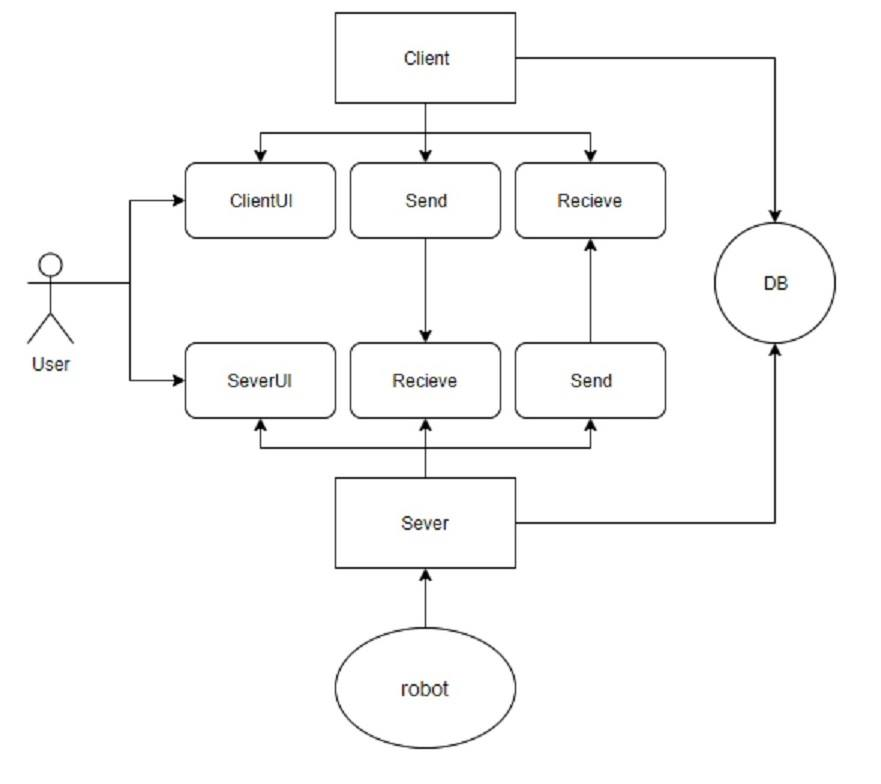
\includegraphics[width=7cm]{structure.jpg}
\end{center}
\caption{It's system structure.}
\label{fig:1}
\end{figure}






\section{User Classes and Characteristics}
$<$\\
(一)、實況收看與線上聊天用戶:該類使用者需要在與其他使用者交流時有好的環境\\
(二)、網路購物使用者或線上查詢用戶:此類使用者提出的問題需要在短時間內被回復\\
$>$

\section{Operating Environment}
$<$Describe the environment in which the software will operate, including the 
hardware platform, operating system and versions, and any other software 
components or applications with which it must peacefully coexist.$>$



\iffalse  %  %
\section{User Documentation}
$<$List the user documentation components (such as user manuals, on-line help, 
and tutorials) that will be delivered along with the software. Identify any 
known user documentation delivery formats or standards.$>$
\section{Assumptions and Dependencies}

$<$List any assumed factors (as opposed to known facts) that could affect the 
requirements stated in the SRS. These could include third-party or commercial 
components that you plan to use, issues around the development or operating 
environment, or constraints. The project could be affected if these assumptions 
are incorrect, are not shared, or change. Also identify any dependencies the 
project has on external factors, such as software components that you intend to 
reuse from another project, unless they are already documented elsewhere (for 
example, in the vision and scope document or the project plan).$>$
\fi   %

\chapter{External Interface Requirements}

\section{User Interfaces}
$<$

\begin{figure}[h]
\begin{center}
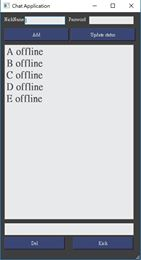
\includegraphics[width=7cm]{interface3.jpg}
\end{center}
\caption{sever interface}
\label{fig:2}
\end{figure}

\begin{figure}[h]
\begin{center}
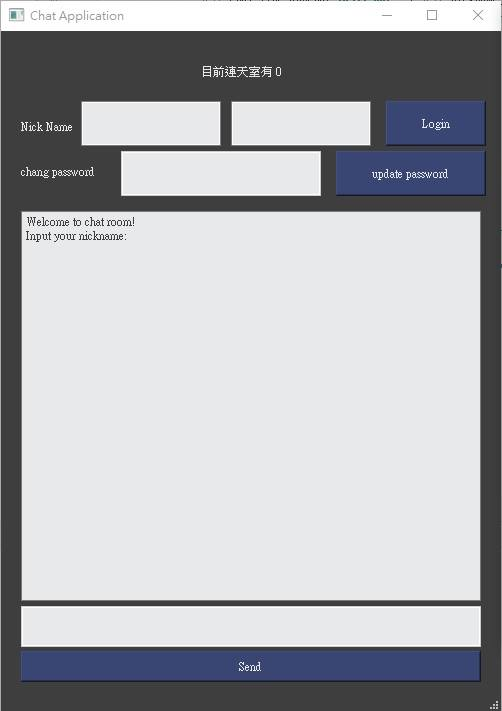
\includegraphics[width=7cm]{interface1.jpg}
\end{center}
\caption{client interface}
\label{fig:3}
\end{figure}
$>$



\section{Software Interfaces}
$<$
	client 與mongo數據庫連接,實時上傳用戶資料\\
	sever  與mongo數據庫連接,處理各個使用者上傳的資料并做回應\\
$>$




\chapter{System Features}
$<$This template illustrates organizing the functional requirements for the 
product by system features, the major services provided by the product. You may 
prefer to organize this section by use case, mode of operation, user class, 
object class, functional hierarchy, or combinations of these, whatever makes the 
most logical sense for your product.$>$

\section{System Feature 1}
$<$Don’t really say “System Feature 1.” State the feature name in just a few 
words.$>$

\subsection{Description and Priority}
$<$Provide a short description of the feature and indicate whether it is of 
High, Medium, or Low priority. You could also include specific priority 
component ratings, such as benefit, penalty, cost, and risk (each rated on a 
relative scale from a low of 1 to a high of 9).$>$

\subsection{Stimulus/Response Sequences}
$<$List the sequences of user actions and system responses that stimulate the 
behavior defined for this feature. These will correspond to the dialog elements 
associated with use cases.$>$

\subsection{Functional Requirements}
$<$Itemize the detailed functional requirements associated with this feature.  
These are the software capabilities that must be present in order for the user 
to carry out the services provided by the feature, or to execute the use case.  
Include how the product should respond to anticipated error conditions or 
invalid inputs. Requirements should be concise, complete, unambiguous, 
verifiable, and necessary. Use “TBD” as a placeholder to indicate when necessary 
information is not yet available.$>$

$<$Each requirement should be uniquely identified with a sequence number or a 
meaningful tag of some kind.$>$

REQ-1:	REQ-2:

\section{System Feature 2 (and so on)}


\chapter{Other Nonfunctional Requirements}

\section{Performance Requirements}
$<$\\(1)系統運行穩定。 \\
(2)系統資料安全。\\ 
(3)用戶端回應快捷,速度能達到業務的基本要求。\\ (4)系統具有一定的容錯和抗干擾能力,在非硬體故障或非通訊故障時,系統能夠保證終端能正 常運行。\\ (5)擴展性強,能夠滿足將來業務和財務擴展需要\\
$>$


\section{Security Requirements}
$<$\\(1)許可權控制 根據不同使用者角色,設置相應許可權,用戶的重要操作都做相應的日誌記錄以備查看,沒有許可權的用 戶禁止使用系統。 \\
(2)重要資料加密 本系統對一些重要的資料按一定的演算法進行加密,如使用者口令、重要參數等。\\
(3)資料備份 允許使用者進行資料的備份和恢復,以彌補資料的破壞和丟失。\\$>$

\section{Software Quality Attributes}
$<$\\(1)記錄日誌 本系統應該能夠記錄系統運行時所發生的所有錯誤,包括本機錯誤和網路錯誤。這些錯誤記錄便於 查找錯誤的原因。 \\
(2)驗證許可權 本系統的所有功能都應該進行功能許可權、部門許可權的判斷和控制。 \\
(3)控制必錄入項
本系統能夠對必須錄入的專案進行控制,使使用者能夠確保資訊錄入的完整。 \\
(4)方便操作 儘量從用戶角度出發,以方便使用本產品。如:錄入資訊時,敲入回車鍵游標的自動跳轉、輸 入法的自動轉換,資訊檢索時輸入漢語簡拼快速檢索到結果等。 \\
(5)用戶可自訂 為了滿足業務的不斷變化,一些重要的參數應該可以靈活設置。\\
$>$


\end{CJK}
\end{document}
